\section{Strategies for traceability of SysML elements}\label{sec:strategies}
\sideboxbegin{o}
This section presents the 4 strategies considered to integrate the functionalities of Trace\textit{a} into SysMLv2.
\sideboxend

During this fourth deliverable we explored  different strategies offered by SysML to allow trustable traceability.

In this section, we present the four strategies considered, their strengths and weaknesses, as well as the one promoted by those in charge of the SST.
This section details the integration of the concepts of trace and trace link within KerML to be able to harness the notions of confidence and justifications (Evidence) of these latter. 
 
\subsection{Root-level adaptations}
\begin{figure}[h]     
	\centering
	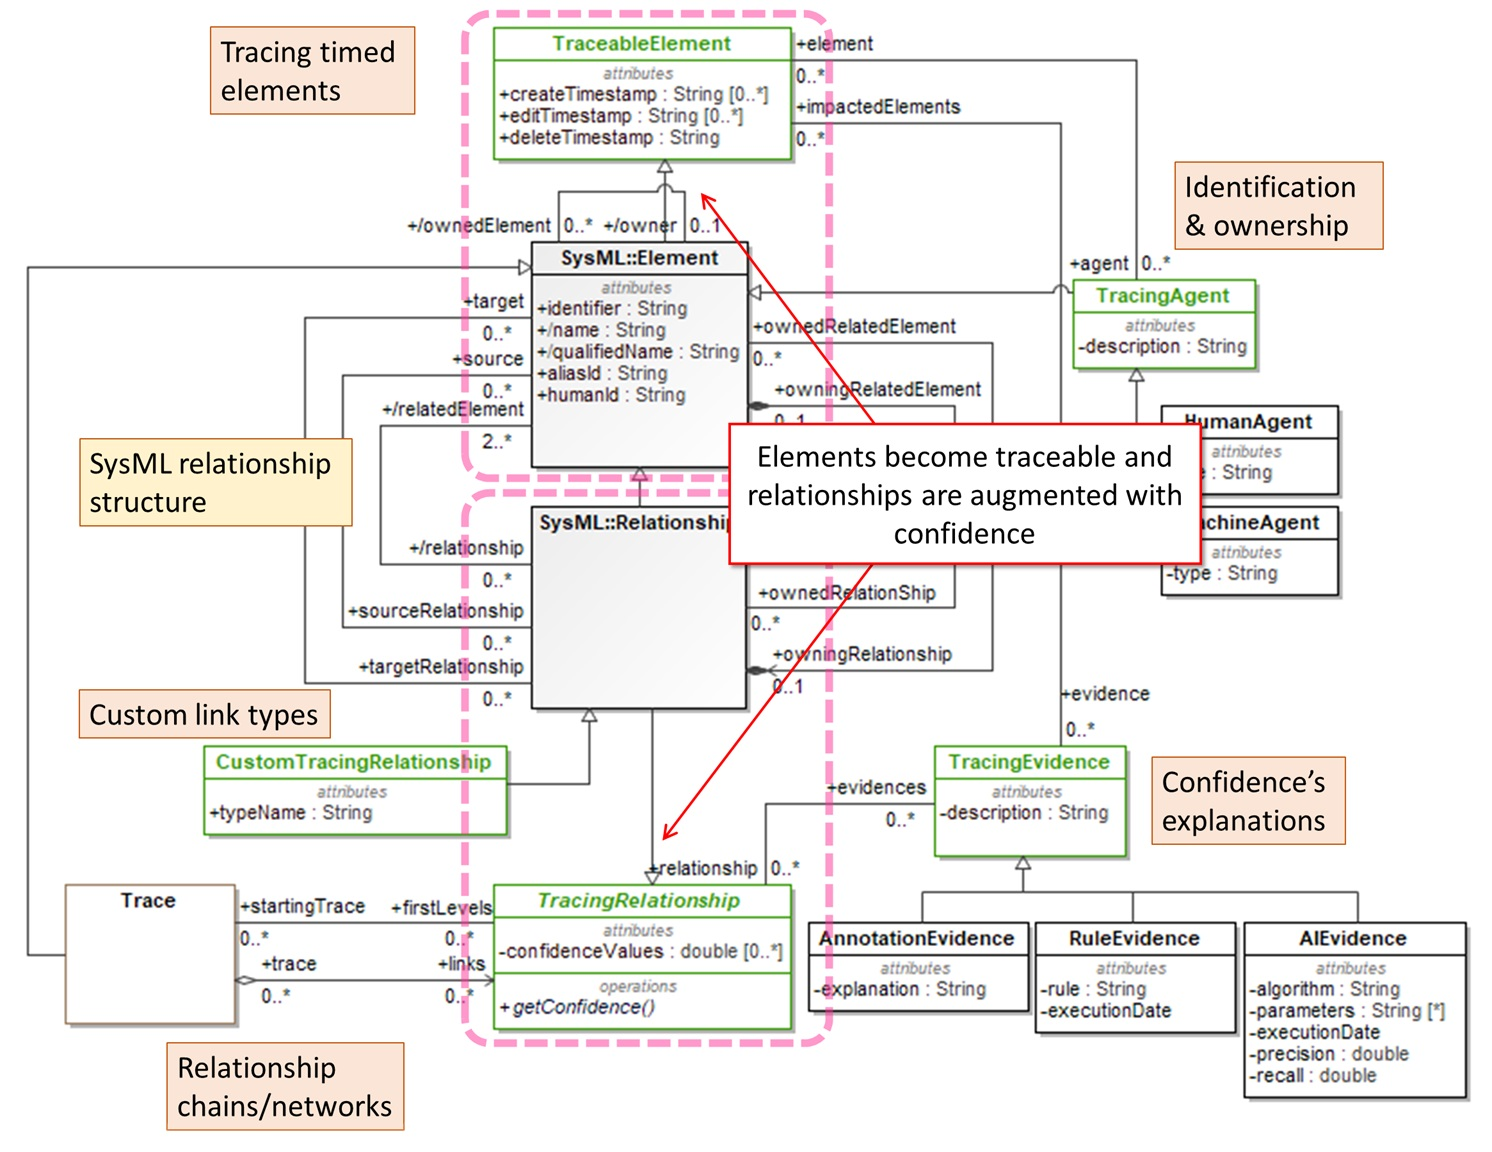
\includegraphics[width=.95\linewidth]{images/strategy1-root.jpg}
	\caption{Adaptation of root-level elements. }
	\label{fig:strategy1}
\end{figure}
The first strategy consists in augmenting the root elements with the attributes necessary for traceability. \Fig{fig:strategy1} shows the modifications required. In gray are the SysML classes, in green the hinge/border classes. The purple dotted lines underline the areas of interest. A TraceableElement class increases the {KerML} Elements by aggregating evolution markers (timestamps) and references to the agents responsible for their identification. The latter are particularly interesting when using non-deterministic algorithms for identifying the tracing links (see the detail of the metamodel of Trace\textit{a} for more details~\cite{batot2021-not-another-metamodel}).
Another class comes to increase the Relationships by attributing to it a value of confidence.

This strategy must have been left because it turns out to be too intrusive in the language. Changing the root elements potentially impacts the entire language structure and therefore could not be incorporated into the KerML/SysMLv2 specification process. Moreover, this strategy implies the definition of a concrete syntax which fits into the {KerML} language schema -- which can be very expensive in terms of consistency evaluation and verification.

\subsection{Annotation type dedicated to tracing}
\begin{figure}[ht]     
	\centering
	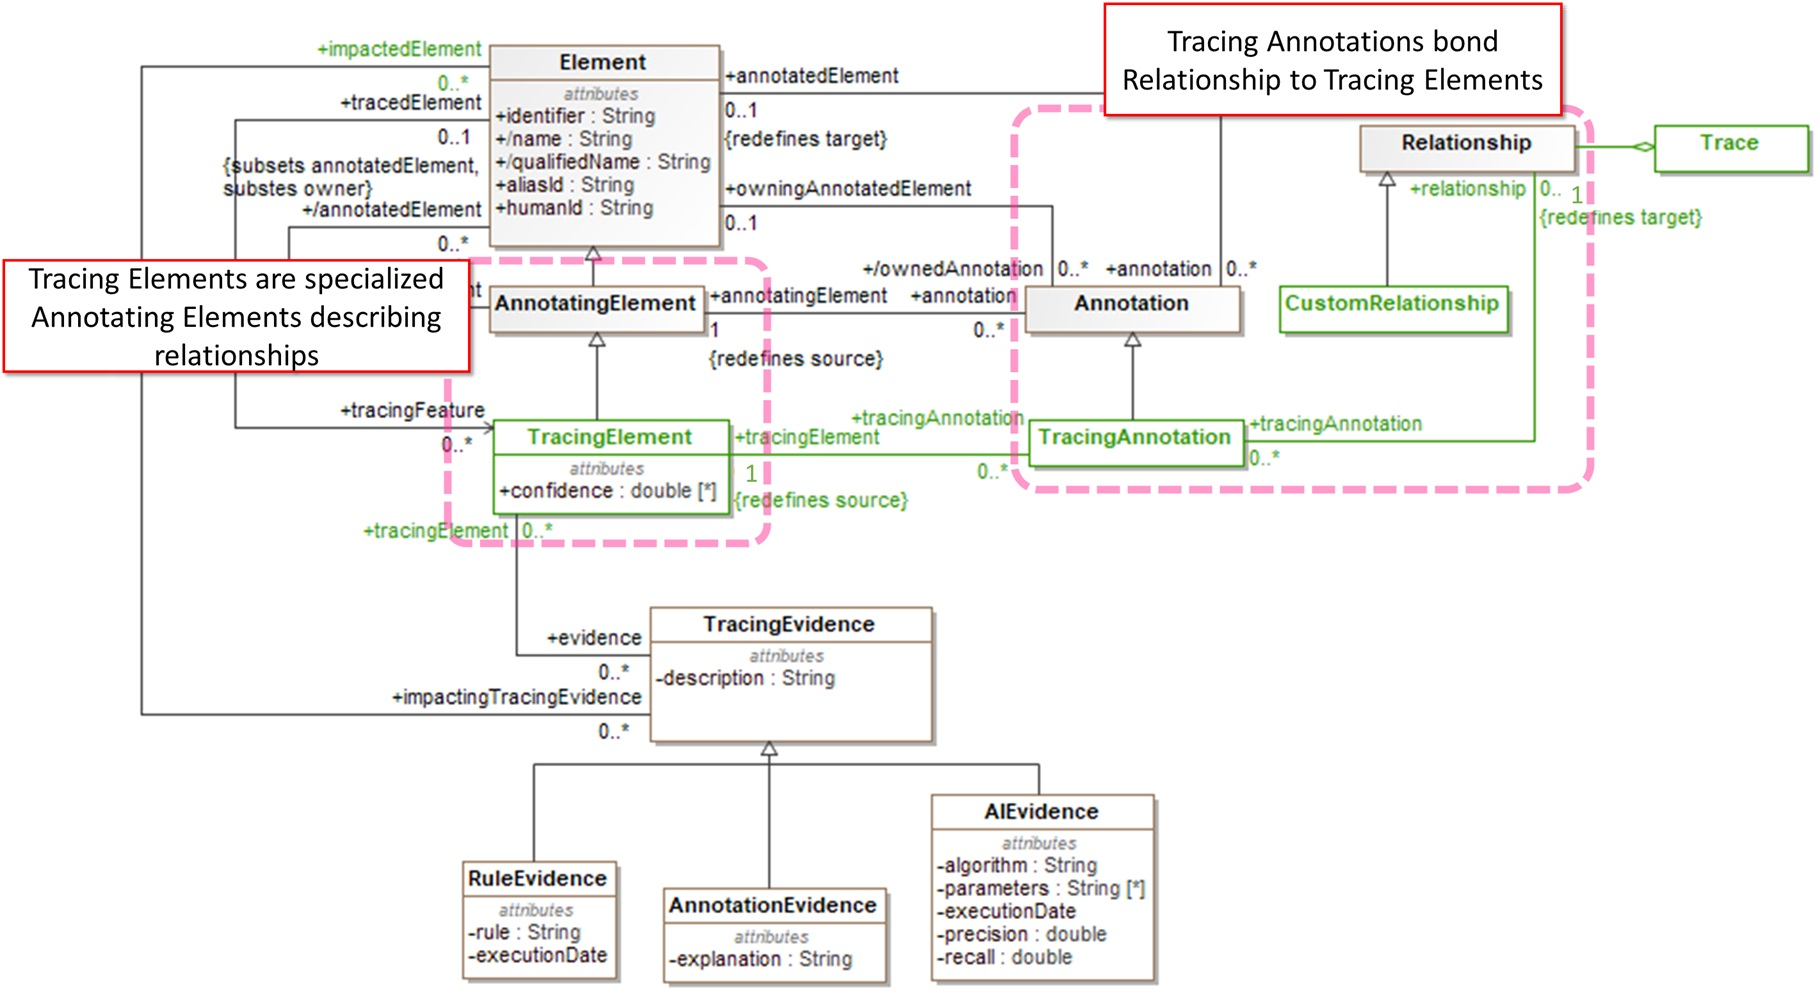
\includegraphics[width=.99\linewidth]{images/strategy2-annotation.jpg}
	\caption{A new type of annotation for {KerML}.}
	\label{fig:strategy2}
\end{figure}
To avoid modifying the fundamental elements of {KerML}, our second idea was to redefine an annotation type dedicated to tracing. To do this, a TracingAnnotation links a Relationship to a TracingElement just as an annotation links an Element to an AnnotatingElement. The idea is to allow the relevant relationships to be annotated with confidence values (and associated with a set of information justifying the calculation of these values). \Fig{fig:strategy2} illustrates the modifications necessary to apply this extension to {KerML}.

This strategy reuses the existing concrete syntax (and to add the keywords necessary to enter the confidence value and the justifications). An illustrative example is provided in Listing~\ref{lst:strategy1}.
However, this strategy poses a problem {in terms of tooling}. Indeed, by modifying the abstract syntax (the metamodel) to add a new type of annotation, all the tools allowing the manipulation of this syntax must be updated.
{This is an intrusive solution again. In a language still in the process of stabilization, the chances of making these changes happen are slim.}
% \vspace{4cm}

\begin{center}
\begin{lstlisting}[caption={Sample of a concrete syntax for tracing annotations},
label=lst:strategy1,
style=mystylesysml,
linewidth=12.5cm,
xleftmargin=4.2cm,
morekeywords={type,confidence,description}]
  trace Req2Source {
     from elt1 to elt2 /** Elements */ 
     type CustomLinkForClasses
     confidence 0.83
     impacts D, E, F
     description "Something"
  }
\end{lstlisting}
\end{center}  


% \vspace{6cm}
Nonetheless, the concept of annotation is to be retained here -- it suits perfectly the idea of traceability \textit{orthogonal} to the software. With tracing annotation, a change in the traced elements does not necessarily impact the tracing elements, and vice versa.



\subsection{A new type of (\textit{annotating feature)}}
\begin{figure}[h]     
	\centering
	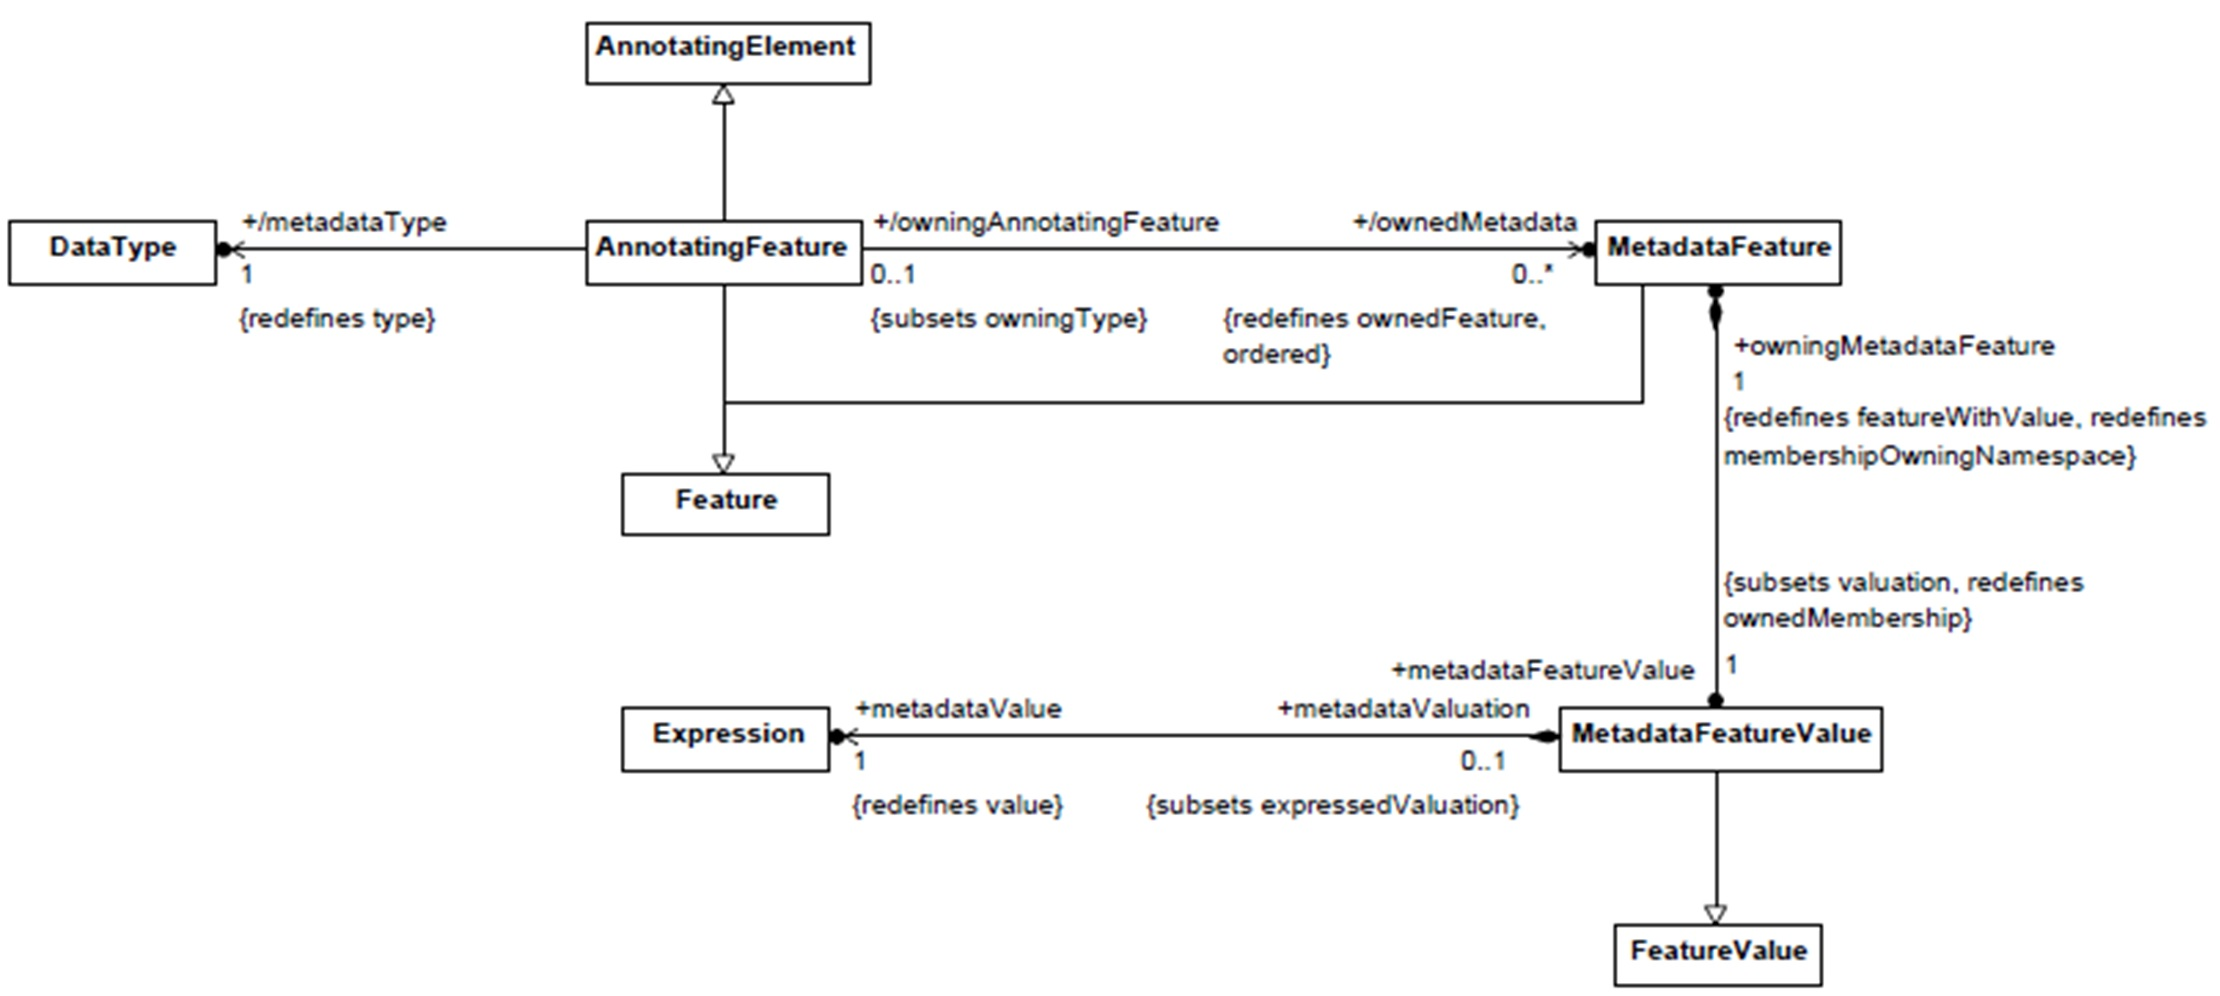
\includegraphics[width=.99\linewidth]{images/kerml-annotatingfeature.jpg}
	\caption{Snippet of the KerML metamodel: AnnotatingFeature and valued Expressions for adaptable metadatatypes.}
	\label{fig:kermlannot}
\end{figure}

\begin{figure}[h]     
	\centering
	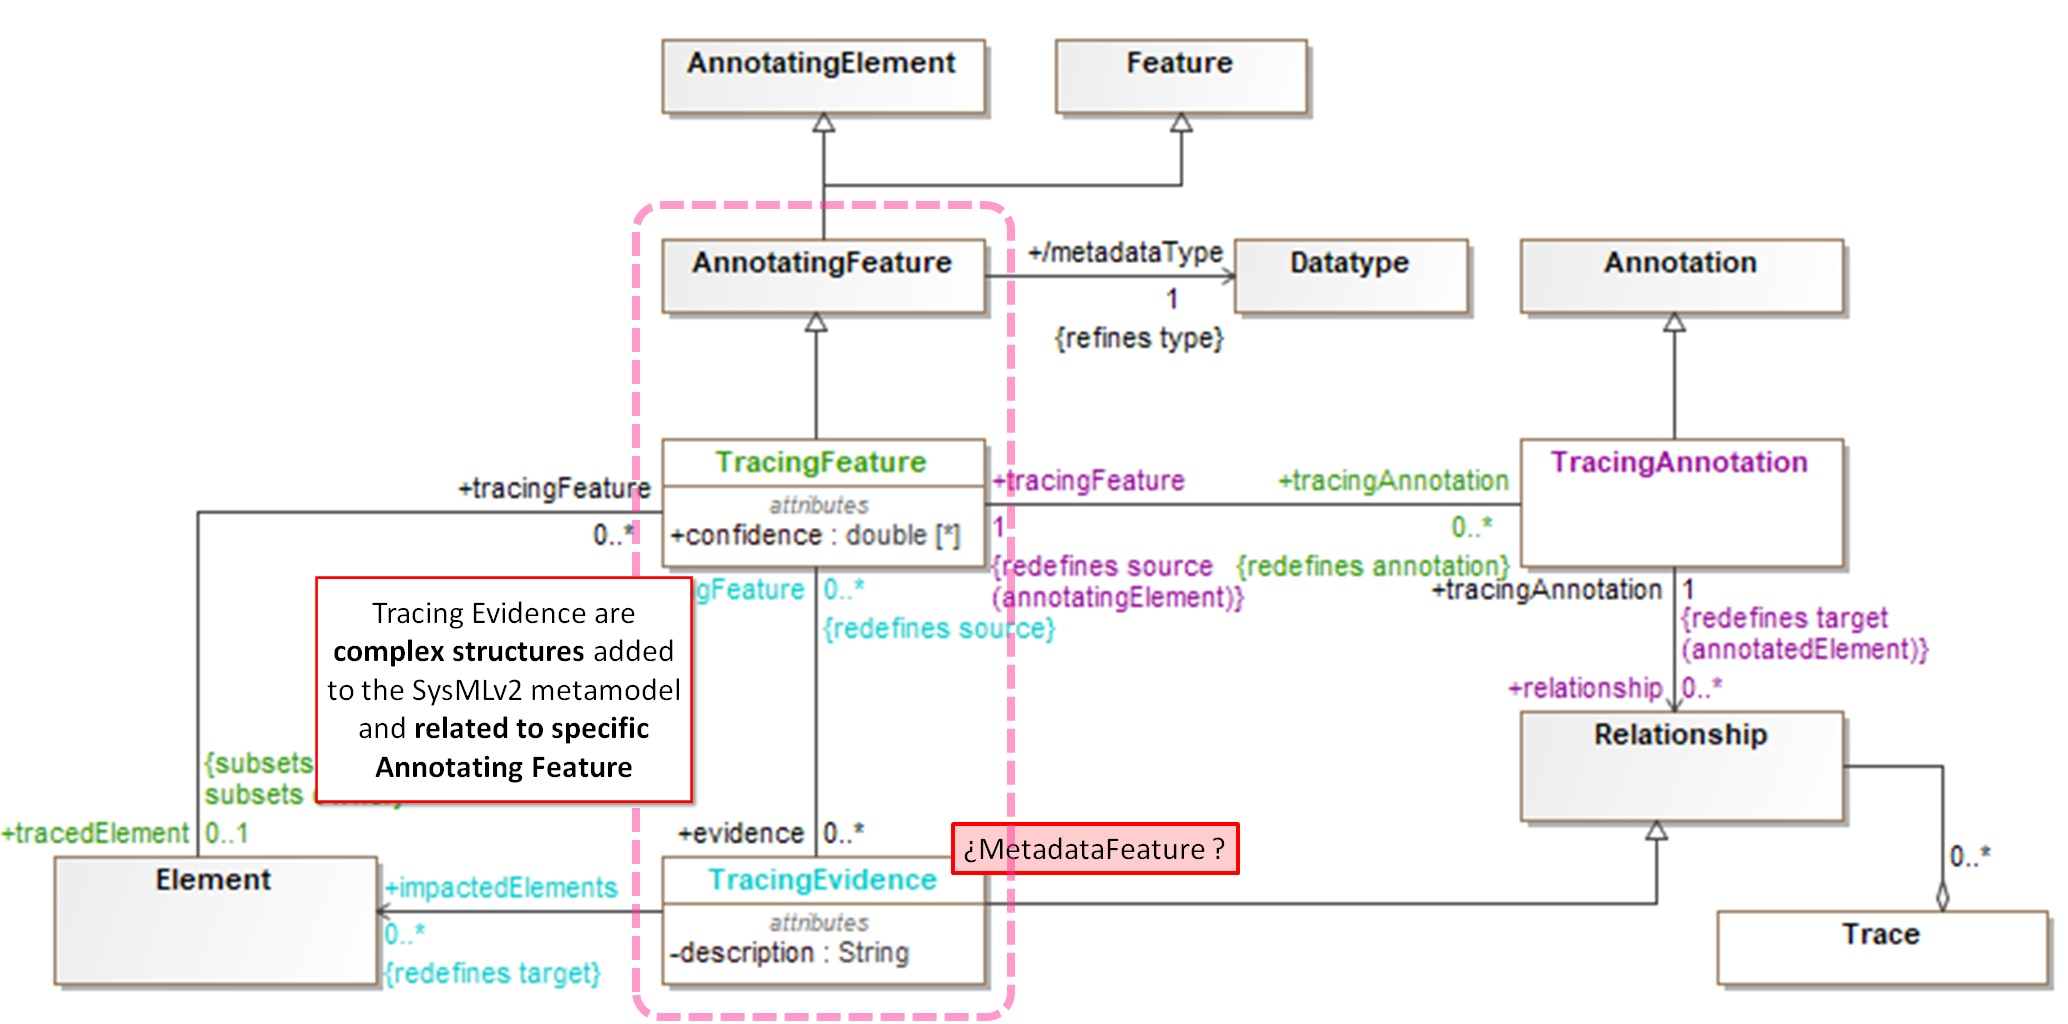
\includegraphics[width=.99\linewidth]{images/strategy3-annotatingfeature.jpg}
	\caption{A new type of annotating feature dedicated to traceability .}
	\label{fig:strategy3}
\end{figure}

The KerML specification states that "\textit{an AnnotatingFeature is a kind of AnnotatingElement that allows the definition of structured metadata with attributes specified by the modeler.}" (KerML specification, p. 178~\cite{kerML}). \Fig{fig:kermlannot} presents a snippet of the KerML metamodel where the AnnotatingFeature class is defined. AnnotatingFeatures use MetadataFeatures which redefine new features for associated elements (respecting the typing defined in DataTypes). These features will be evaluated at the \textit{execution of expression at model level} and a value will be associated with each feature.

\Fig{fig:strategy3} shows the modifications to be made to {KerML} to allow the redefinition of a new type of AnnotatingFeature dedicated to traceability.
A TracingAnnotation associates a TracingFeature with a Relationship. This Feature includes a level of confidence and possibly evidence (references to other elements).



This approach is the most interesting. KerML / SysMLv2 maintainers informed us that this "AnnotatingFeature / Datatype" structure is in their sights because it allows the addition of functionality in the form of metadata libraries without directly modifying the language elements (what we call "orthogonality" ). More precisely, they plan to use only this type of annotation and to ban its refinement in favor of this structure to allow the simplified writing of specialized function libraries (\textit{feature libraries}).
From September 2021, the different types of AnnotatingElement (Comment, TextualRepresentation and AnnotatingFeature) will converge to a representation based on AnnotatingFeature. This migration will simplify, first of all, the elaboration of comments specific to a project / domain thanks to the use of dedicated Datatypes.

% \pagebreak
\subsection{A feature library for traceability }
The last strategy considered will be the one implemented. Instead of modifying the abstract syntax structure of {KerML} (\textit{i.e.,} metamodel level), the idea is to create a library of features dedicated to traceability (model level).
It is about redefining datatypes specific to the tracing features in order to join them to the structures concerned at the model level. It is an orthogonal method comparable to the use of \textit{stereotypes} in UML. The comparison is based on the ability offered by the AnnotatingFeature to define new (libraries of) features without altering the base of the language itself. The process is particularly suited to building a tracing strategy, often implemented \textit{after} the software has been put into production.

\vspace{3em}
The Listings \ref{lst:featurelibrary1} and \ref{lst:featurelibrary2} present our feature library {in SysML}. Listing~\ref{lst:featurelibrary1} contains the library declaration; Listing~\ref{lst:featurelibrary2} contains an example of application of such datatype  defined on a concrete example. It illustrates the allocation of a confidence value of 0.7 to a connection between a requirement (req) and a package. The second case (line 16 to 20) attributes a description and points to an element impacted (by the evaluation of the confidence),
% \vspace{10cm}

\begin{center}
\begin{lstlisting}[caption={Definition of a datatype dedicated to traceability (partial listing).},
label=lst:featurelibrary1,
style=mystylesysml,
linewidth=15cm,
xleftmargin=2.2cm,
morekeywords={part,filter}]
 package TracingAnnotations {
	attribute def ConfidenceTracing {
		attribute confidence : Real;
		attribute impact : Anything[*]
		assert constraint 
		  { confidence >= 0.0 && confidence <= 1.0 } 
	}
	 
	attribute def ExplainableTracing {
		attribute description : String;
		attribute evidence : Evidence;
		attribute agent : Agent;
	}  
 }
\end{lstlisting}
\end{center}  

\begin{center}
\begin{lstlisting}[caption={Use of metadata features for traceability},
label=lst:featurelibrary2,
style=mystylesysml,
frame=shadowbox,
rulesepcolor=\color{blue},
linewidth=15cm,
xleftmargin=2.2cm,
morekeywords={confidence,description,evidence,impact, part, req,package}]
 import package TracingAnnotations::*;

 /*Definition of the target system. */
 part vehiculetest {}
 req RE01_MLV {}
 package UMLCD_CORE {}

 /*Assignment of a confidence of 0.7 to the Req2Design link.*/
 connection Req2Design connect RE01_MLV to UMLCD_CORE {
   @ConfidenceTracing {
     confidence = 0.7;
   }
 }
 
 /*Assigning a description and an impact to the Req2Design link.*/
 connection Req2Design connect RE01_MLV to UMLCD_CORE {
   @ExplainableTracing {
     description = "Something";
     impact = (vehiculetest);
   }
 }
 
\end{lstlisting}
\end{center}


% 
\begin{center}
\begin{lstlisting}[caption={Confidence and evidences for trustable traceability},label=lst:relationship,style=mystylextext,frame=shadowbox, rulesepcolor=\color{blue}]
Relationship  returns SysML::Relationship :
    'relationship' Identification?
    RelationshipRelatedElements
    RelationshipBody;

OwnedRelationship returns SysML::Relationship :
    'relationship' Identification?
    'to' RelationshipTargetList
    RelationshipBody;

fragment RelationshipRelatedElements 
            returns SysML::Relationship :
    'from' RelationshipSourceList ( 'to' RelationshipTargetList )?
  | 'to' RelationshipTargetList;

fragment RelationshipSourceList returns SysML::Relationship :
    RelationshipSource ( ',' RelationshipSource )*;

fragment RelationshipSource returns SysML::Relationship :
    source += [SysML::Element | QualifiedName];

fragment RelationshipTargetList returns SysML::Relationship :
    RelationshipTarget ( ',' RelationshipTarget )*
;

fragment RelationshipTarget returns SysML::Relationship :
    target += [SysML::Element | QualifiedName];

fragment RelationshipBody returns SysML::Relationship :
    ';' | '{' RelationshipOwnedElement* '}';

fragment RelationshipOwnedElement returns SysML::Relationship:
      ownedRelatedElement += OwnedRelatedElement
    | ownedRelationship += OwnedDocumentation
    | ownedRelationship += OwnedTextualRepresentationAnnotation;

OwnedRelatedElement returns SysML::Element :
      'element' ( humanId = Name )? ElementBody
    | OwnedRelatedRelationship;

OwnedRelatedRelationship returns SysML::Relationship :
    'relationship' ( humanId = Name )? RelationshipBody;
\end{lstlisting}
\end{center}

